\documentclass{beamer}
\usepackage[english]{babel}
\usepackage[utf8]{inputenc}
\usepackage[T1]{fontenc}
\usepackage{stmaryrd} %http://www.ctan.org/pkg/stmaryrd
\usepackage{amsmath} %http://www.ctan.org/pkg/amsmath
\usepackage{amssymb}
\usepackage{subfig}

\usetheme[usetitleprogressbar, numbering=fraction]{metropolis}

\newcommand\bb{Benjamin Boisson}
\newcommand\gc{Guillaume Combette}
\newcommand\dl{Dimitri Lajou}
\newcommand\vl{Victor Lutfalla}
\newcommand\om{Octave Mariotti}
\newcommand\mr{Raphaël Monat}
\newcommand\me{Etienne Moutot} % He is not the only one author o/ Just that \em is already taken
\newcommand\js{Johanna Seif}
\newcommand\ps{Pijus Simonaitis}




\title{Blend'it}
\subtitle{Integrated project}
\author{\bb\\ \gc\\ \dl\\ \vl\\ \om\\ \mr\\ \me\\ \js\\ \ps\\}
\date{April 15th, 2016}

\begin{document}
\maketitle

\begin{frame}
\tableofcontents[
  currentsection,
  sectionstyle=show/show,
  subsectionstyle=hide/hide]
\end{frame}




\bgroup
\setbeamercolor{background canvas}{bg=black}
\begin{frame}[plain]{}
\end{frame}
\egroup

\begin{frame}{}
  Blend'it = Crowd animation and Environment generator (two images from the project).
\end{frame}

\section{What is Blend'it ?}
\begin{frame}{What is Blend'it ?}
  Blend'it is a \textbf{Blender plug-in} for \textbf{crowd animation} and \textbf{environment generation}.
  
  + screenshot
\end{frame}

\begin{frame}{A Lot of Powerful Software}

% \begin{figure}
%   \centering
%   \subfloat[Goalem\label{fig:a}]{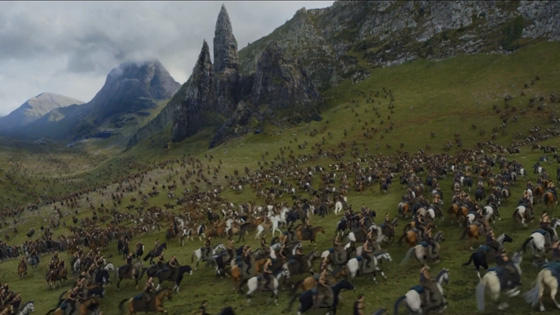
\includegraphics[width=5cm]{golaem.jpg}}\qquad
%   \subfloat[Massive\label{fig:b}]{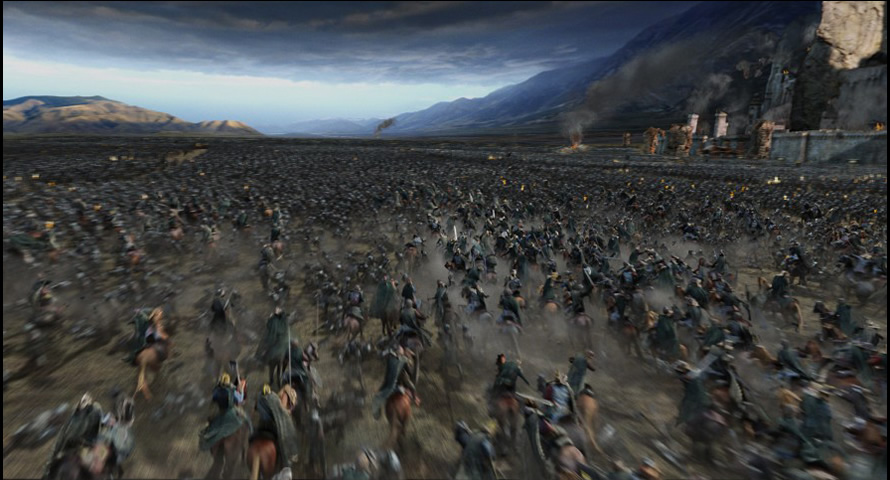
\includegraphics[width=5cm]{massive.jpg}}
% \caption{A lot of Powerful Software}
% \label{fig:1}
% \end{figure}
\begin{figure}
  \includegraphics<1>[width=.95\textwidth]{golaem.jpg}
  \includegraphics<2>[width=.95\textwidth]{massive.jpg}
  \caption{\only<1>{Golaem}\only<2>{Massive}}
\end{figure}

\end{frame}

\begin{frame}{A Lot of Expensive Software}
  \begin{itemize}
    \item Maya3D: 
    \item Golaem: 5000\$/year
    \item Massive: 3,500 - 16,000\$/year
  \end{itemize}
\end{frame}

\begin{frame}{Why Blender ?}
  \begin{itemize}
    \item Strong open-source basis
    \item Powerful python API (no need to modify the source code of blender)
  \end{itemize}
\end{frame}

\begin{frame}{Project organization}
  Diagram of two subprojects
\end{frame}

\section{Algorithms}
\begin{frame}{Crowd animation - }
  bla
\end{frame}

\begin{frame}{Crowd animation - }
  bli
\end{frame}

\section{Implementation}
\begin{frame}{Crowd animation - }
  bla
\end{frame}

\begin{frame}{Crowd animation - }
  bli
\end{frame}

\bgroup
\setbeamercolor{background canvas}{bg=black}
\begin{frame}[plain]{}
\end{frame}
\egroup
\end{document}
